\chapter{PRELIMINARIES}
\label{sec:Preliminaries}

FSMs are mathematical abstractions for real word systems. When an FSM gets an input, it moves from one state to another with an output. Since synchronizing sequences consider only the destination state without making any observation on the system, the output is not in the scope of this work. Therefore, we can consider an FSM as an automaton with a simple transition function and without an output.

When an automaton is complete and deterministic, it is defined by a triplet ${\cal A}=(S, \Sigma, \delta)$  where $S = \{1, 2, \ldots, n\}$ is a finite set of $n$ states, $\Sigma$ is a finite alphabet consisting of $p$ input symbols (or simply {\em letters}), and $\delta : S \times \Sigma \rightarrow S$ is a total transition function. When the transition function is a partial function, then the automaton is said to be a {\em partial} automaton.

If the automaton ${\cal A}$ is at a state $s$ and if an input $x$ is applied, then ${\cal A}$ moves to the state $\delta(s,x)$. Figure~\ref{fig:inv}~(left) shows an example automaton ${\cal A}$ with 4 states and 2 input.

\begin{figure}[ht]
	\centering
	\includegraphics[width=0.9\textwidth]{figs/inverse.pdf}
	\caption{A synchronizing automaton ${\cal A}$~(left), and the data structures to store and process the transition function $\delta^{-1}$  in memory (right). For each symbol $x \in \Sigma$, we used two arrays ${\tt ptrs}$ and ${\tt ids}$ where the former is of size $n + 1$ and the latter is of size $n$. For each state $s \in S$, ${\tt ptrs}[s]$ and ${\tt ptrs}[s+1]$ are the start~(inclusive) and end~(exclusive) pointers to two ${\tt ids}$ entries.  The array ${\tt ids}$ stores the ids of the states $\delta^{-1}(s,x)$ in between ${\tt ids}$[{$\tt ptrs$}[$s$]]  and ${\tt ids}$[{$\tt ptrs$}[$s+1$] - 1].}
	\label{fig:inv}
\end{figure}

\pagebreak

An element of the set $\Sigma^\star$ is called an {\em input sequence} (or simply a {\em word}). $|w|$ denotes the length of $w$, and $\varepsilon$ expresses the empty word. The transition function $\delta$ can be extended to a set of states and to a word in the usual way. Assuming $\delta(s,\varepsilon)=s$, for a word $w \in \Sigma^\star$ and a letter $x \in \Sigma$, $\delta(s,xw) = \delta(\delta(s,x),w)$. Likewise, for a set of states $S' \subseteq S$, $\delta(S',w) = \{ \delta(s,w) | s \in S'\}$.

The inverse $\delta^{-1} : S \times X \rightarrow 2^S$ of the transition function $\delta$ is also a well defined function; $\delta^{-1}(s,x)$ denotes the set of states with a transition to state $s$ with input $x$. Formally, $\delta^{-1}(s,x) = \{ s' \in S | \delta(s',x)= s\}$.  Figure~\ref{fig:inv}~(right) shows the data structure used to store the inverse transition function for the example automaton.

Let ${\cal A}=(S, \Sigma, \delta)$, $C \subseteq S$ and $C^{\langle 2 \rangle} = \{ \{ s_i, s_j \}| s_i,s_j \in C \}$ be set of multisets  with cardinality two. For $\{ s_i, s_j \} \in C^{\langle 2 \rangle}$, if $s_i=s_j$ then it is called a \textit{singleton}, otherwise called a \textit{pair}. 

An automaton which is produced from the set of pairs $S^{\langle 2 \rangle}$; ${\cal A}^{\langle 2 \rangle}=(S^{\langle 2 \rangle},\Sigma,\delta^{\langle 2 \rangle})$ is called the \textit{pair automaton}. For a pair automaton, the set of inputs is the same and the transition function of the pair automaton is $\delta^{\langle 2 \rangle}(\{ s_i,s_j \},x) = \{ \delta(s_i,x), \delta(s_j,x) \}$. 

\begin{figure}[ht]
	\centering
	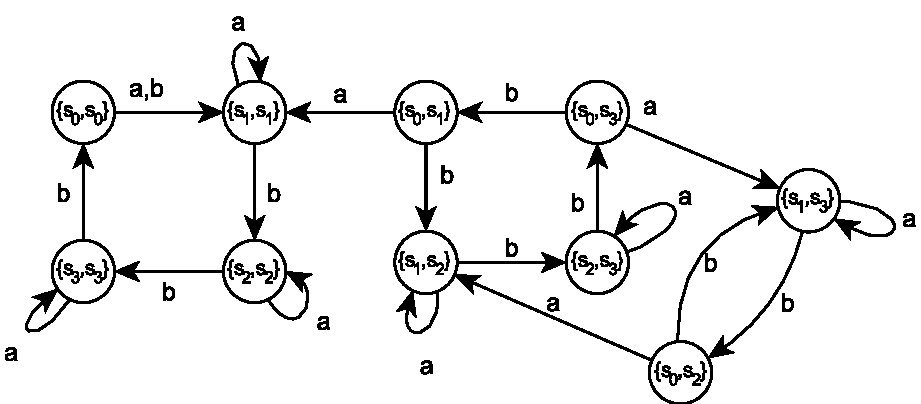
\includegraphics[width=\textwidth]{figs/pair.pdf}
	\caption{The pair automaton ${\cal A}^{\langle 2 \rangle}$ of the automaton in Figure \ref{fig:inv}.}
	\label{fig:pair}
\end{figure}

Let $C \subseteq S$ be a set of states and $w \in \Sigma^*$ be an input sequence.  If the cardinality of $\delta(C,w)$ is one then $w$ is said to be a \textit{merging sequence} for $C$. If there exists a merging sequence for a set of states $C$, then $C$ is called \textit{mergeable}. If there exists a merging sequence $w$ for $S$ (i.e. for all states), $w$ is called a \textit{reset word}\footnote{In the literature, reset word is also called as both synchronizing word and synchronizing sequence. In this thesis, these three terms are used interchangably.} of the automaton, and the automaton is called {\em synchronizable} or {\em synchronizing}. As shown by \cite{Eppstein90}, deciding if an automaton is synchronizing can be performed in time $O(pn^2)$ by checking if there exists a merging word for $\{ s_i, s_j \}$, for all  $\{ s_i, s_j \} \in S^{\langle 2 \rangle}$. Recently, Berlinkov \cite{Berlinkov2016} showed that there exists an algorithm that decides on synchronizability in linear expected time in $n$. 

\v{C}ern\'y has conjectured that the length of the shortest synchronizing word of an automaton with $n$ states is at most $(n-1)^2$~\cite{cerny}. \v{C}ern\'y has also provided the following class of automata ${\cal A}_c$, called {\em \v{C}ern\'y automata}, which hits to this conjectured upper bound. 


Let ${\cal A}_c=(S, \Sigma_c, \delta_c)$, $\Sigma_c = \{a, b\}$, $|S| = n$, and 
\[
  \delta_c(s_i, x) = \left.
  \begin{cases}
    s_{(i+1)\ \mathrm{mod}\ n}, & x = b \text{ or } s_i = s_0\\
    s_i, & \text{otherwise}
  \end{cases} \right.
\]

An example of a \v{C}ern\'y automaton is given in Figure~\ref{fig:inv}.

\section{Graphics Processing Units and CUDA}\label{sec:gpu}

At the hardware level, a CUDA capable Graphics Processing Units~(GPU) processor is a collection of
\textit{multiprocessors} (SMX), each having a number of
\textit{processors}.  Each multiprocessor has its own shared memory
which is common to all its processors.  It also has a set of
registers, texture memory (a read only memory for the GPU), and
constant (a read only memory for the GPU that has the lowest access
latency) memory caches.  In any given cycle, each processor in the
multiprocessor executes the same instruction on different data.
Communication between multiprocessors can be achieved through the
\textit{global device memory}, which is available to all the
processors in all multiprocessors~\cite{nvidia}.

In the software level, the CUDA model is a collection of threads
running in parallel.  The programmer decides the number of threads
to be launched.  A collection of threads, called a \textit{warp},
run simultaneously (on a multiprocessor).  If the number of
threads is more than the warp size then these threads are time-shared
internally on the multiprocessor.  At any given time, a \textit{block}
of threads runs on a multiprocessor.  Therefore threads in a block may
be bundled into several warps.  Each thread executes a
piece of code called a \textit{kernel}.  The kernel is the core code
to be executed on a multiprocessor.  During its execution, a thread
$t_i$ is given a unique ID and during execution thread $t_i$ can
access data residing in the GPU by using its ID.  Since the GPU memory
is available to all the threads, a thread can access any memory
location.  During GPU computation the CPU can continue to operate.
Therefore the CUDA programming model is a hybrid computing model in
which a GPU is referred as a co-processor (\textit{device}) for the
CPU (\textit{host}).
